% !TeX spellcheck = en_US
\documentclass[]{TAACpaper}
\usepackage[linesnumbered,boxed]{algorithm2e}
\begin{document}

%This is the comment. Further under the text features of use of style of theses are described

%We are specifying language of the paper
\selectlanguage{english}
\def\dd#1#2{\frac{\partial#1}{\partial#2}}
\section{
%%%%%%%%%%%%%%% You have to specify name of your paper here
``Investigation of tuning parameters of tabu search algorithm and its modification  for solving the static Routing Courier Delivery Problem.'' 
}

\authors{
R.~Shafeyev , L.~Lyubchik 
}

\abstract{
%%%%%%%%%%%%%%% You have to insert abstract of your paper here

The paper considers the routing courier delivery problem with the service time for which the discrete model was constructed and the calculation scheme based on tabu search algorithm. The efficiency  of the proposed algorithm‘s scheme has been tested on a large-scale problems, which were generated on the basis of different classes known model routing problems.

}

%%%%%%%%%%%%%%% To define new section use a command \subsection
% We are defining "Introduction" here
\subsection{Introduction}
%%%%% Paragraph text. To separate paragraphs use empty lines.
In the research we consider a static vehicle routing problem with time windows. This variant of the routing problem is a common problem in the courier delivery industry. Effective solution to this problem affects the quality of services provided by the company, as well as the magnitude of potential losses caused by the excess of the agreed terms of delivery. The proposed solution to the problem is based on the automation of the process of planning the route and involves the use of distributed information systems for the possible implementation of these approaches in practice. Another important criterion for good transport plan are low transport costs, which affect the cost of services.

The Routing Courier Delivery Problem with time windows requires that a set of vehicles satisfy a collection of customer requests. Each client request requires the use of a single vehicle to receive and load a specified amount of goods at one source location(sender) and to deliver them to destination location(receiver). All requests must be performed without violating either the vehicle capacity or the customer time window. The solution is a master plan that solves the problem, and takes into account the daily events that take place according to plan. In this paper, we present a discrete model and a modified tabu search algorithm  to solve the  Courier Delivery Problem with time windows. 

In order to validate our strategies decisions technique effectiveness, we have constructed a new set of benchmark problems for the pickup and delivery problem with time windows based on which were generated on the basis of different classes known model routing problems. Computational results substantiate the solution quality and efficiency of our modified tabu search algorithm.
 

\subsection{Problem Statement}
Let $C,dim(C)=n$ is a set of vehicles and $Q,dim(Q)=m$ is a set of requests received from customers at the current time.

Suppose that the following information is known about vehicles from set $C$: \\
$\vec{P}_c$ -- vehicle position, $c \in C$;\\
$L_c$ -- vehicle capacity, $c \in C$.

Let $S$ is a set of senders, ($dim(S) = dim(Q) = m$), $R$ is a set of receivers, $dim(R) = dim(Q) = m$. Then each client request $q \in Q$ includes the following information:\\
$s_q$ -- a sender of client shipment, $s \in S$; \\
$r_q$ -- a receiver of client shipment, $r \in R$; \\
$\vec{P}_{s_q}$ -- sender position;\\
$\vec{P}_{r_q}$ -- receiver position; \\
$w_q$ -- client shipment that is required to deliver from the sender to the recipient; \\
$[t_{s}^{q}, t_{s}^{q}+ \Delta{t_{s}^{q}}]$ -- the time window within which worker must to pick up the goods from the sender;\\ 
$[t_{r}^{q}, t_{r}^{q}+ \Delta{t_{r}^{q}}]$ -- the time window within which worker must deliver the goods to the receiver.
 
Thus, each application can be represented as a tuple:
\begin{equation}
\forall q \in Q: \exists q = (s_q,r_q, \vec{P}_{s_q}, \vec{P}_{r_q}, w_q, t_{s}^{q}, \Delta{t_{s}^{q}}, t_{r}^{q}, \Delta{t_{r}^{q}})
\end{equation}
To estimate the cost of transportation between destinations defined cost function $\Omega$:
\begin{equation}
\forall i,j \in S \cup R: \exists \Omega_{i,j} = \Omega(\vec{P}_i,\vec{P}_j)
\end{equation}

Necessary to construct the optimal routes of vehicles movement for the transportation of goods from the sender to the receiver for all client requests.

\begin{figure}[h]
	\hfil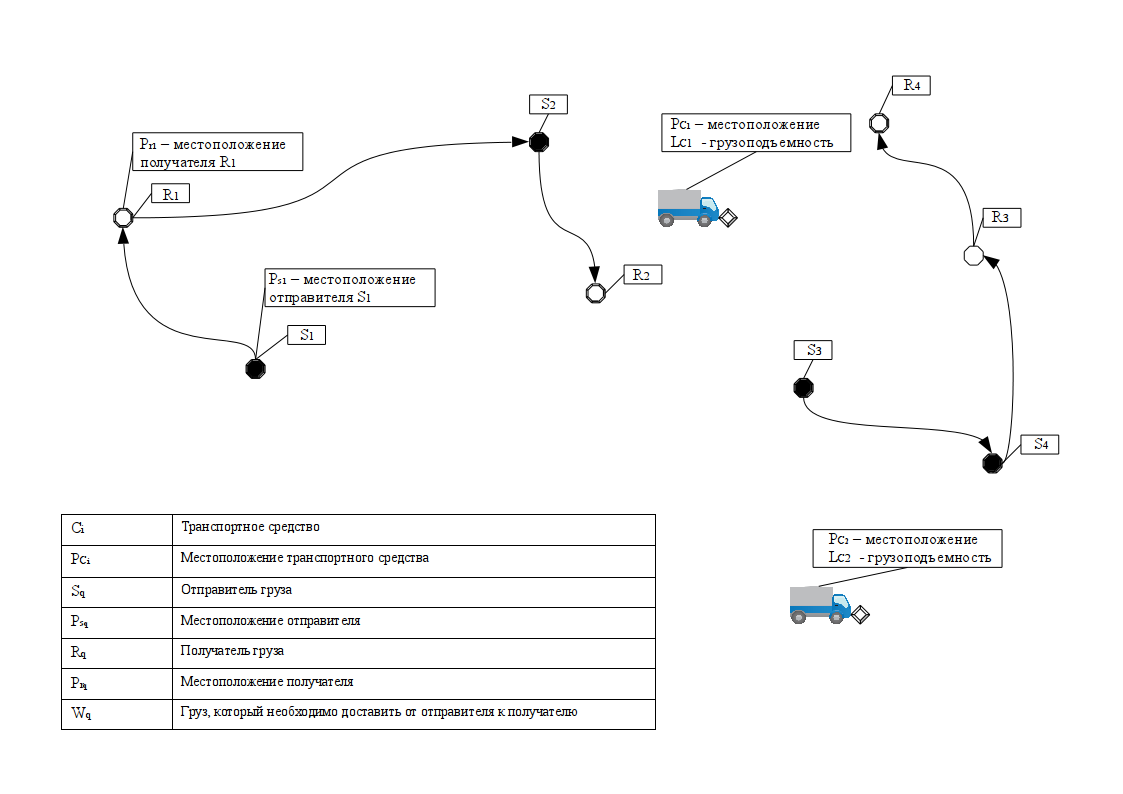
\includegraphics[height=4.0in]{images/scheme}\hfil
	\caption
	{
		Example of the Routing Delivery Problem.
	}
	\label{aba:fig1}
\end{figure}

\subsection{Discrete model}
Routing problem can be represented as a directed graph $G=G(V,E)$. The set $V=C\cup{S}\cup{R}$ -- nodes of the graph $G$, consisting of elements of vehicles, senders and receivers. $E$ -- dynamic set of arcs of the graph $G$, such that:
\begin{equation}
\forall e(X) \in E: e(X) = (v_i,v_j), \exists v_i \in V, v_j \in V/C
\end{equation}

Let $X = \{X^k\}^n_{k=1}$ is a sequence of variable matrices for each vehicle $k \in C$. Elements of the matrices take the following values:
\begin{equation}
  x^{(k)}_{i,j} = 
    \begin{cases}
	  1,&\text{the vehicle $k \in C$ moves from $i$ node to the $j$}\\
	  0,&\text{otherwise.}
    \end{cases}
\end{equation}
where: $i\in{V/C \cup {k}}, j \in V/C$.

Let us introduce the vector  of variables $ \vec{Y}  ^ k(X) $ for each vehicle $ k \ in C $. Vector elements have the following values:
\begin{equation}
\vec{y}^{(k)}_{j}(X) = 
\begin{cases}
1,&\text{the request $j \in Q$ is processed by vehicle $k \in C$}\\
0,&\text{otherwise.}
\end{cases}
\end{equation}
where: $i\in{V/C \cup {k}}, j \in V/C$.


Let $t^k_j(X^{(k)})$ -- arrival time of the vehicle $k \in C$ at the destination $j \in S \cup R$. 

The objective function takes the following form:
\begin{equation} \label{main_objective}
  F(X) = 
    \sum_{k \in C}
     \sum_{i,j\cup{V}} 
     \Omega_{ij} \cdot x_{ij}^{(k)} 
     \to min
\end{equation}

We define constraints on the objective function (\ref{main_objective}), which provided the continuity of routes:
\begin{align} 
& \sum_{k \in C}\sum_{j \in S \cup R}x^{(k)}_{i,j} \leq 1, 
\forall i \in V \label{main_cond_1}\\
& \sum_{k \in C}\sum_{i \in S \cup R \cup \{k\} } x^{(k)}_{i,j} = 1, 
\forall j \in S \cup R \label{main_cond_2}\\
& \sum_{i \in S \cup R \cup \{k\} } x^{(k)}_{i,\omega} - 
\sum_{j \in S \cup R} x^{(k)}_{\omega,j} \leq 1, 
\forall \omega \in S \cup R,  \forall k \in C \label{main_cond_3}\\
&  \sum_{i \in S \cup R / Z}\sum_{j \in Z } x^{(k)}_{i,j} > 0, 
Z=\{z \in Z: \sum_{j \in S \cup R}x^{(k)}_{j,z}>0 \}  ,\forall k \in C \label{main_cond_4}
\end{align}

The restriction (\ref{main_cond_1}) prohibits to a node in the graph $G$ has more than one output arc. The restriction (\ref{main_cond_2}) prohibits to a node has more than one input arc.  The constraint (\ref{main_cond_3}) indicates that the number of input arcs to the node can not be less than the output arcs (this constraint considers the fact that the vehicle can leave the destination only if it has visited this node). The restriction (\ref{main_cond_4}) excludes local loops.

Then next constraints synchronize values of variables $X$ and $\vec{y}$ for each request $q \in Q$ and prohibits the service of receiver before a visit to the sender:
\begin{align} 
& x^{(k)}_{s_q} + x^{(k)}_{r_q} = 2 \cdot y^{(k)}_{q}(X), \forall k \in C, q \in Q  \\
& y^{(k)}_{q}(X) \cdot (\tilde{t}^k_{r_q}(X^{(k)})-\tilde{t}^k_{s_q}(X^{(k)})\ge{0}, \forall k \in C, q \in Q
\end{align}

Define restrictions for accounting of vehicle capacity and time windows:
\begin{align} 
& \sum_{j\in{Q}} \omega_j \cdot y_{j}^{k} \leq L_k, \forall{k}\in{C}\\
& t_{s}^{q} \leq \tilde{t}^k_{s_q}(X^{(k)} \leq t_{s}^{q}+ \Delta{t_{s}^{q}}, \forall q \in Q, \label{tws_cond} \\
& t_{r}^{q} \leq \tilde{t}^k_{r_q}(X^{(k)} \leq t_{r}^{q}+ \Delta{t_{r}^{q}}, \forall q \in Q, \label{twr_cond}
\end{align}



\subsection{Description of the Algorithm}
Present the set of matrices $\{X^k\}$ in the form of a vector defined on the hypercube $E^\eta=\{0.1\}^\eta$, where $\eta=n\cdot(2m+1)\cdot 2m$. The aim of the task is to minimize the objective function:
\begin{align} 
& F(\vec{u})\to min,\vec{u}\in E^{\eta}
\end{align}	

Denote by $\delta(\vec{u},\vec{v})$ the Hamming distance between $\vec{u}$ and $\vec{v}$. Through $N_l(\vec{u})$ we denote the neighborhood of a point $\vec{u}$ radius $l$, ie:
\begin{align} 
& N_l(\vec{u})=\{\vec{v} \in E^{\eta}:\delta(\vec{u},\vec{v})\le l \}, l=\bar{1,\eta}
\end{align}	

When $l=\eta$ a set $ N_l(\vec{u})$ for any vector $\vec{u}$ coincides with the set $E^{\eta}$ and being in this neighborhood vector with a minimum value of the objective function is equivalent to solving the original problem. The standard algorithm local search algorithm starts with a randomly selected vector $\vec{u^0}$.
On the $i$ step of the algorithm move from the current vector in the neighbouring that the minimum value of the objective function in the neighborhood of the given vector:
\begin{align} 
& F(\vec{u}^{i+1})=min\{F(\vec{v}):\vec{v} \in N_l(\vec{u}^i)\}
\end{align}	

The algorithm terminates at a local optimum, when $F(\vec{x^{i+1}})=F(\vec{x^i})$. When solving the transportation problem is a typical situation when many local optimums and only one of them is global:
\begin{align} 
& F_{opt}=min\{F(\vec{v}):v \in E^{\eta}\}
\end{align}	

To ensure that the algorithm did not stop in a local minimum, and passed from one local minimum to another, with edges removed the Central point and when searching for the minimum of the following rule applies. Let $l=2$ and in the transition from $\vec{u^{i+1}}$ to $\vec{u^i}$ change the values in the coordinate $(u_\lambda^{i}, u_\omega^{i})$. The algorithm stores such pair for the last $h$ couple of steps and in the next step prohibits the movement in these directions. An ordered list of such pairs
\begin{align} 
& \phi^i=\{(u_\lambda^{i},u_\omega^{i}),(u_\lambda^{i-1},u_\omega^{i-1}),\cdots,(u_\lambda^{i-h+1},u_\omega^{i-h+1}) \} 
\end{align}	
called the list of prohibitions. When building the list of all pairs of different and a pair of $(u_\lambda,u_\omega),\lambda \ne \omega$ does not prohibit the movement of pairs $(u_\lambda,u_\lambda)$ and $(u_\omega,u_\omega)$. When $l>2$ similarly constructed three coordinates, fours, etc. A set of non-restricted vectors denote by $N_l(\vec{u^i},\vec{\phi^i})$. In order that the search was effectively, it is advisable to use small values $h$ and to control this parameter in the course of the algorithm.

\begin{algorithm}[H]
	\textbf{function TabuSearch}($u^0,l,p,h$) \\
	// Initialize variables:	\\
	$u^{opt} = u^0$
	$F^{opt} = F^0$
	$\phi^{0} =  \emptyset$
	$i=0$ \\
	\While{the breakpoint is not triggered }{
	   $N_l = N_l(u^i,\phi^i,p,h) $ \\
		\eIf{$N_l \ne   \emptyset $}{
			$ u^{i+1} = u^i$ \\
			$i = i + 1$ \\
			\textbf{goto} 5
		}
		{
			// find optimum into the neighbord $N_l$: \\
			$ u^{i+1} : F(u^{i+1}) = min\{ F(y): y \in N_l \}$
		} 

		\If{$F(u^{i+1}) < F_{opt})$}{
			$ F_{opt} = F(u^{i+1})$ \\
			$ u^{opt} = u^{i+1}$
		}
			
		
		$\phi^{i+1} = update(\phi^i)$\\
		i = i + 1\\
	   
	}
	\textbf{return} $u^{opt}$
	
\caption{Pseudo-code for probabilistic tabu-search algorithm.}
\label{alg:TabuSearch}
\end{algorithm}

Denote by $N_l(\vec{u^i},\vec{\phi^i},p)$ probabilistic edge that goes from a deterministic $N_l(\vec{u^i},\vec{\phi^i})$ as follows. Each vector $\vec{v} \in N_l(\vec{u^i},\vec{\phi^i})$ with probability $p$ included in the neighborhood $N_l(\vec{u^i},\vec{\phi^i},p)$ regardless of other points. Note that this set may be empty or contain only one point. The General scheme of the probabilistic search algorithm with a list of prohibitions referred to as pseudo-code in algorithm \\
scheme \ref{alg:TabuSearch}.

As the stopping criterion is based on the total number of steps $N_stop$, in the course of which does not change the value $F_{opt}$. Values $l,p,h$ are the control parameters of the algorithm. Their choice depends on the problem dimension.

In the presented scheme, it was assumed that the value of $h$ (the dimension of the deny list) does not change in the course of the algorithm. This creates certain difficulties in the implementation of the scheme, as it is unknown how long is to take a list of prohibitions. At small $h$ the algorithm can start walking cycle. At large $h$ the search becomes inefficient. One of the simple rules regulating the length of the list of prohibitions is the following.

If at the next step of the algorithm, the edge  $N_l(\vec{u^i},\vec{\phi^i},p)$ turned out to be empty, it is added to the list of fictitious vector $\vec{0}$. This vector nothing forbids, but reduces the number of bans per unit.

\subsection{Initialization}
To use a search algorithm is restricted by the need to build the initial solution. To obtain the initial solution $\vec{u^0}$ you can use a heuristic method to construct the route. The essence of these methods is the following. Every car has consistently built a route by adding another is not considered clients according to specified rules.

The most known method of construction of the route proposed by Solomon in 1987 year and found in the literature as a method of Solomon. This algorithm is fast enough (computational complexity $O(n^3)$, therefore, it is useful to initialize a vector $\vec{u^0}$.

At the beginning of the algorithm, you add one to a customer on the route according to time limits. The choice of the first client is randomly or chosen one, you want to serve first. Then, each valid client $u$ from the set of outstanding clients $Q^{'}$ (the set $Q^{'}\subset{Q}$) evaluated insertion between two adjacent nodes route. For selection of inserts used criterion:
\begin{align} 
& c(v_i,u,v_i+1)=[\min_{p=2,\dots,n^k}(\Omega_{p-1,u}^k+\Omega_{u,p}^k-\mu \Omega_{p-1,p}^k) ]
\end{align}	
where:

$k$ - vehicle route $k\in C$;
$n^k$ - the number of nodes in the route;
$\mu$ - arbitrary parameter, $\mu \ge 0 $.

Added the client, which is $c(v_i,u,v_i+1)$ least:
\begin{align} 
& u^*:c(v_i,u^*,v_i+1)=min[c(v_i,u,V_i+1)]
\end{align}	

As a result the client $u^*$ is added to the current route $k$ the position between nodes $v_i$ and $v_i+1$.

\subsection{A Method of Forming Solutions Neighborhood}
The most difficult part of the local search algorithm with the prohibitions are viewing the surroundings $N_l(\vec{u^i},\vec{\phi^i})$ of the current point $\vec{us^i}$. For even larger values of $l$ and the parameter $p=1$ in the outskirts plenty of points. But due to the nature of the model's constraints many of them are not the solution. Therefore, due to the nature of the considered discrete tasks, we used the following method of determining the area. On the $i$ step of the algorithm compiled from routes pair: $\{R_1,R_2\},\{R_1,R_3\},\dots,\{R_1,R_n\},\{R_2,R_1\}, \{R_2,R_3\},\dots,\{R_2,R_n\},\dots,\{R_{n-1},R_{n}\}$. Then over each pair of routes is performed in moving requests. The resulting displacement vectors $\vec{u}$ are neighborhood $N_l(\vec{u^i},\vec{\phi^i})$. For moving  we used change-move  and swap-move operations.


\subsection{Analysis of the algorithm parameters}
Modified tabu search algorithm has 3 main parameters: $p$ -- the probability of hitting solutions in a neighborhood, $h$ -- size of the list of prohibitions and $N_{neighbors}$ -- accepted count limit of size of neighbordhood $N_l(\vec{u})$. For the experiments, we constructed the test tasks on the basis of the capacity routing problems developed by Breedam, Fisher, Christofides and Eilon. To determine trends in time and cost of the decision to use exponential smoothing by a factor of $0.1$.

\begin{figure}[h]
	\hfil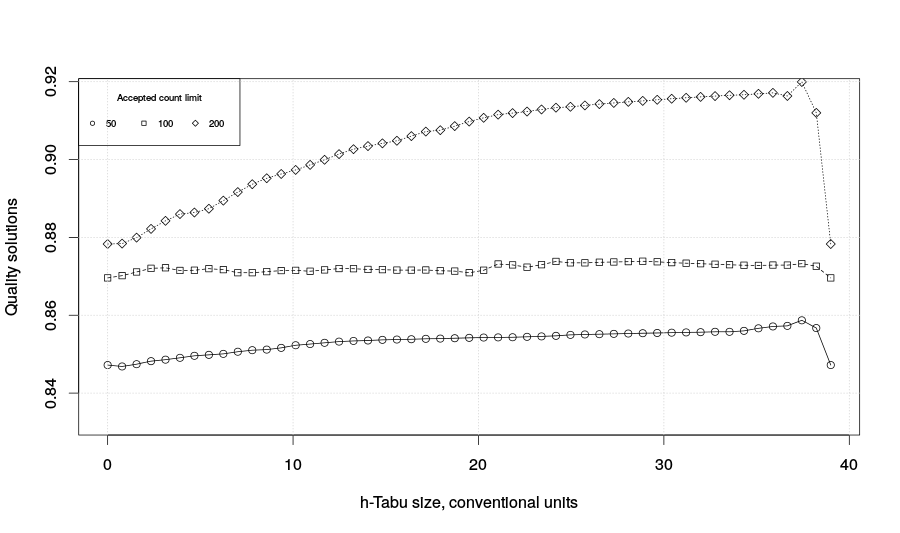
\includegraphics[height=3.0in]{images/tabuSize_stepCount}\hfil
	\caption
	{
	  The dependence of the quality of solutions on the size of the tabu list when using $ StepCount $ termination strategy
	}
	\label{aba:fig2}
\end{figure}

In the first computational experiment we made finding the best solutions for different values of the tabu size parameter $h \in [0, 40]$ (pict. 1 an pict. 2). In this experiment we use two different breakpoint strategies: 
\begin{enumerate}
	\item $StepCount$ termination strategy --  terminates when an amount of steps has been reached;
	\item $TimeMillisSpent$ termination strategy -- terminates when an amount of time has been used.
\end{enumerate}

As should have been expected, for large values of the parameter a jam occurs in local optimum due to the large number of restrictions of movement in space. Otherwise if you select a too small tabu size, algorithm can still get stuck in a local optimum. 
\begin{figure}[h]
	\hfil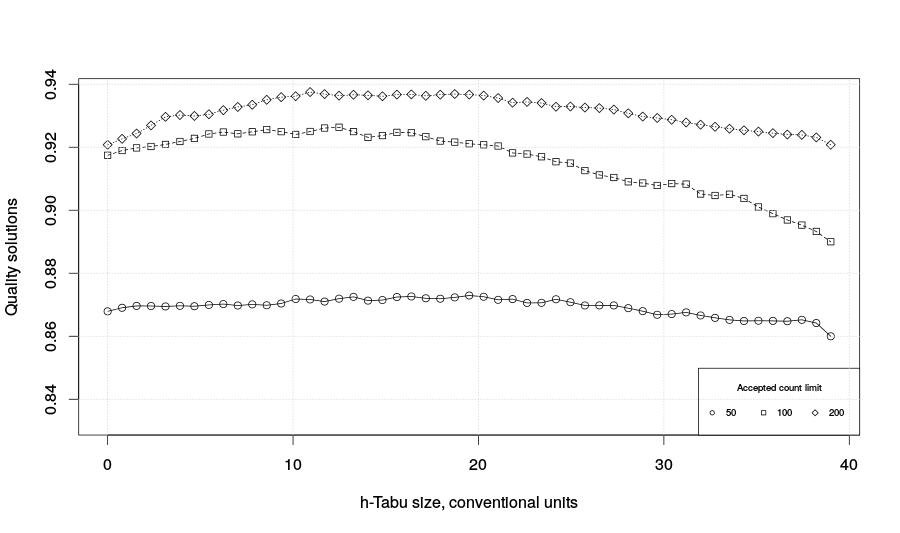
\includegraphics[height=2.0in]{images/tabuSize_time}\hfil
	\caption
	{
	  The dependence of the quality of solutions on the size of the tabu list when using $ TimeMillisSpent $ termination strategy
	}
	\label{aba:fig3}
\end{figure}

In the second experiment we built a relationship between the number $N_{neighbors}$ of viewed solutions neighborhood $N_l(\vec{u})$ using $TimeMillisSpent$ termination strategy. 
\begin{figure}[h]
	\hfil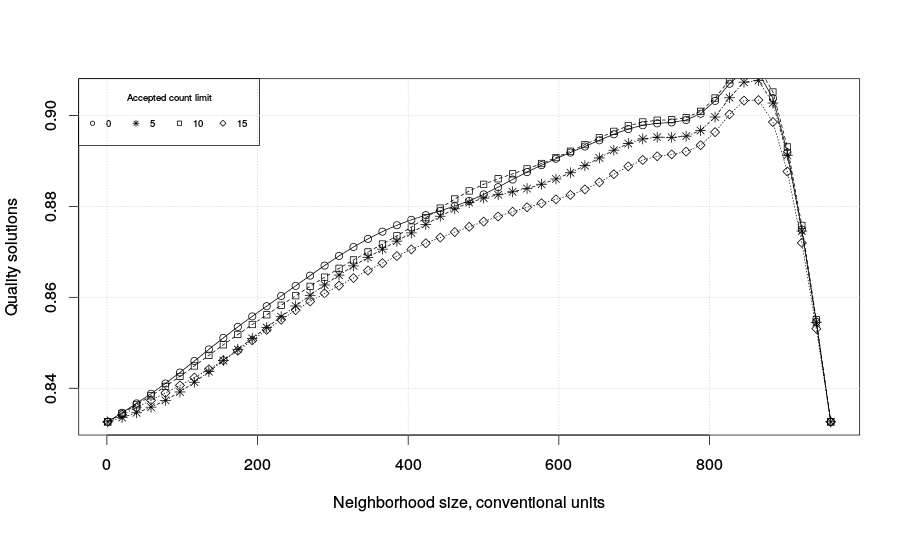
\includegraphics[height=2.0in]{images/acceptedCountLimit}\hfil
	\caption
	{
	  The dependence of the quality of solutions on the neighborhood size when using $ TimeMillisSpent $ termination strategy
	}
	\label{aba:fig4}
\end{figure}


\subsection{Modification}

The first generalized diagram is as follows. First, the set of solutions is constructed by Solomon. Then every solution is improved by tabu search and choose the best solution according to the objective function.

Modification of the scheme is based on the hypothesis of "On a large valley." According to this hypothesis, the average local optima are located much closer to the global than a randomly chosen point. There is a certain concentration of local optimum in a small part of the feasible region, which is figuratively called a large valley. If this assumption is true, then it is advisable to remember the best solutions and based on them design new original decision. We use this idea to solve the  Routing Courier Delivery Problem.

We proceed to the description of the algorithm in scheme \ref{alg:constructSolution}. Let $U^{opt}$ is a sorted array of optimal solutions by value of the objective function ascending,  ie:
\begin{equation} \label{u_sorted}
F(u^{opt}_1) \leq F(u^{opt}_2) \leq \ldots < F(u^{opt}_i) \leq \ldots \leq F(u^{opt}_{sizeof(U^{opt})})
\end{equation}
Each solution $u^{opt}_i$ gets into the population with a given probability $p^i_u$, the probability of selection decreases with increasing sequence number:
\begin{equation} \label{p_sorted}
p^1_u = 1 > p^2_u > \ldots > p^i_u> \ldots   > p^{sizeof(U^{opt})}_u,  p^{sizeof(U^{opt})}_u > 0
\end{equation}

\begin{algorithm}[H]

	\textbf{function constructSolution}( $U^{opt}, p_u, n^{min}_s$) \\
	// $U^{opt}$ -- a sorted set array optimal solutions \\
	
	
	\If{$ sizeof(U^{opt}) <  n^{min}_s$}{
		// construct solution using heuristics(for example, Solomon alg.)\\
		$u^0 = heuristicsConscruction()$ \\
		\textbf{return} $u^0$
	}
	
	\While{$i < sizeof(U^{opt})$}{
		\If{$random(0.0,1.0) > p^i_u$}{
		   i = i + 1 \\
		   \textbf{goto} 8
		}
		$R_i = $randomly select a route from $u^{opt}_i$ solution;
		$u^0 = u^0 \cup R_i$
		i = i + 1\\
		
	}
	
	\If{$u^0 is not complete$}{
	   	$u^0 = heuristicsConscruction(u^0)$
	}
	
	\textbf{return} $u^0$
	
	\caption{Pseudo-code for heuristics construction algorithm.}
	\label{alg:constructSolution}
\end{algorithm}

It then crosses solutions by the following rule: with the first solution is randomly selected route $R_1$. Then another solution is selected from a route $R_2$ that does not include client requests from the first  route etc. If the client requests were not included in the solution $u^0$, then these requests are added by the construction heuristics algorithm (for example, Solomon algorithm).


Now we describe the primary function $SolveCDP()$ of the modified algorithm presented in pseudocode form in Scheme \ref{alg:modTabuSearch}. In this function using a loop is a sequential formation of an array of the best solutions $U^{opt}$ by means TabuSearch algorithm.   

Based on the results of the experiments described in the preceding section, we decided to set the parameters of the algorithm are not fixed values, but as a random variable of predetermined period. For example, the size of the tabu list $h$ is defined as the interval $[10,35]$(see pict. \ref{aba:fig2} and  pict. \ref{aba:fig3}) and the neighbordhood size $l=N_{neighbordhood}$ is defined as the interval $[600\cdot n,850\cdot n]$, where $n$ -- problem size (see pict. \ref{aba:fig4} ).

Let $\vec{\psi_i} = (\psi^1_i,\psi^2_i,\psi^3_i) = (\tilde{l_i},\tilde{p_i},\tilde{l_h})$ -- a set of values of the TabuSearch configuration parameters which was using for solving the problem in the step $i$.

Let $[\psi^j_{begin}, \psi^j_{end}]$ -- an optimal interval of the TabuSearch $j$ -parameter. (For example: if $j=3$, then: $[\psi^3_{begin}, \psi^3_{end}]= [h_{begin}, h_{end}] = [10, 40] $). These intervals are initial data and they are set in the initialization block. 

The configuration parameters  $\psi^j_i $ are randomly selected from the interval $[\psi^j_{begin}, \psi^j_{end}]$ according to a distribution law. We proposed to build the distribution density $f_j(\psi^j_i)$ of the random variable $\psi^j_i$ as follows. At first, we define anchor points:
 
 \begin{equation} \label{anchor_points}
     \rho^j_i =  \dfrac{F(u^{opt}_1)}{avg[F(u^{opt}_k)]}, \forall k: \psi^j_k = \psi^j_i
 \end{equation}
 The number of anchor points $n_{\rho}$  is smaller than the set of optimal solutions, because a set of reference anchor points are removed the same point $(n_{\rho} \leq  n_u)$.
 
The main idea is that the distribution density should be larger at those points (parameters $\psi^j_i$) in which high quality solutions than the points at which the low quality of solutions.
Therefore, we presented the distribution function $f_j(z)$ as a sum of kernel functions:
 \begin{equation} \label{dist_density}
 f_j(z) = \alpha_j * \sum\limits_{i=1}^{n_{\rho}}  \rho^j_i * K(z -  \psi^j_i)
 \end{equation}
 where: $K(x)$ -- kernel function, $ \alpha$ -- a normalizing parameter
 
 We have chosen as the kernel the function of parabolic type(known as an Epanechnikov function),  because during the experiments the best results were obtained using this function:
 \begin{equation} \label{dist_density}
  K(z) = 3/4 \cdot (1-z^2)
 \end{equation}
 

\begin{algorithm}[H]
	\textbf{function SolveCDP}( $n^{min}_s$) \\
	// Initialize variables:	\\
	
	$\psi = \emptyset$,
	$p_u = \emptyset$,
	$U^{opt} = \emptyset$,
	$i=0$ \\
	
	\While{the breakpoint is not triggered }{
		// set TabuSearch parameters \\
		\For{$j=1 \ldots 3$}{
	  	// $f_j$ -- the density distribution of the random \\
	  	// variable $\psi^j$ (TabuSearch parameter $l,p $ or $ h$) \\
	  	$\psi^j_i = random(\psi^j_{begin}, \psi^j_{end}, f_j) $
	  	}
	  	
		// Make solution using euristics construction algorithms \\
		$u^0 = constructSolution(U^{opt} ,n^{min}_s)$ 
		
		// Improve solution $u^0$ using TabuSearch algorithm 
		$u^{opt}_i = TabuSearch(u^0, \vec{\psi_i})$ \\
		
		$U^{opt}  = U^{opt} \cup \{u^{opt}_i\}$ \\
		
		// Sort ascending optimums $U$ of the objective function \\
		$U^{opt} = sort(U^{opt})$\\
		$p^{i+1}_u = update(p^i_u)$\\
		
		i = i + 1\\
		
	}
	\textbf{return} $u^{opt}_1$
	
	\caption{Pseudo-code for modified tabu-search algorithm.}
	\label{alg:modTabuSearch}
\end{algorithm}

 The parameter $\alpha_j$ was introduced in the density function to perform the normalization condition:
 \begin{equation} \label{norm_cond}
 \int\limits_{\psi^j_{begin}}^{\psi^j_{end}} f_j(z)dz = 1  =>  (\alpha_j)^{-1} = \sum\limits_{i=1}^{n_{\rho}} \rho^j_i \cdot  \int\limits_{\psi^j_{begin}}^{\psi^j_{end}} K(z -  \psi^j_i) dz 
 \end{equation}

 The parameter $\alpha_j$ can be written in explicit form:
  \begin{equation} \label{norm_cond}
 \begin{split}
 (\alpha_j)^{-1} & = \dfrac{3}{4} \cdot \sum\limits_{i=1}^{n_{\rho}} \rho^j_i \cdot [(1 - (\psi^j_i)^2) \cdot (\psi^j_{end} - \psi^j_{begin}) + \\
 & + \psi^j_i \cdot ((\psi^j_{end})^2 - (\psi^j_{begin})^2) - 1/3 \cdot (\psi^j_{end})^3 - (\psi^j_{begin})^3)]
 \end{split}
 \end{equation}
 
 In figure \ref{aba:fig5} the results of an experiment in which  were presented a dependence of the quality of the solutions obtained by the classical and modified algorithms and  the breaking point time. As seen from the graph, with an increase in operating time of the computational scheme, the quality of solutions obtained using the modified algorithm is growing faster than using classical Tabu Search algorithm.
 
 \begin{figure}[h]
 	\hfil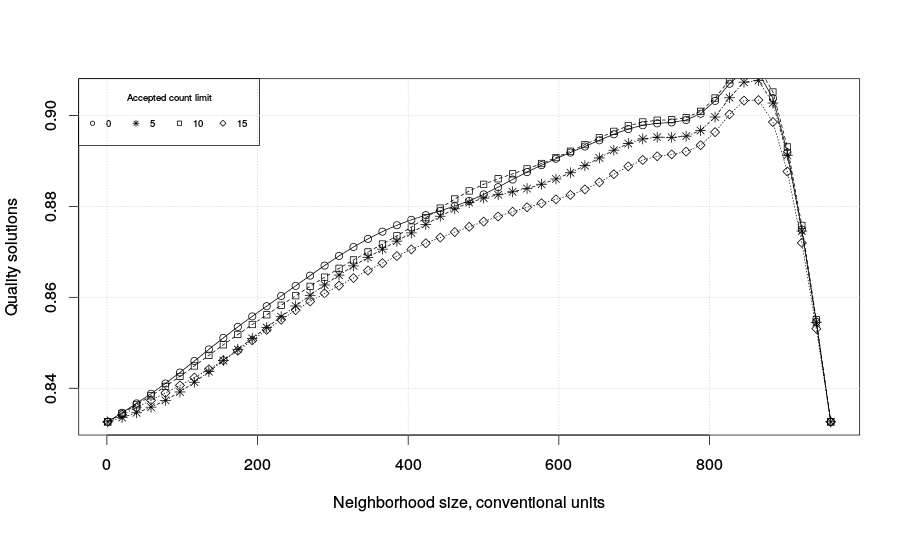
\includegraphics[height=2.0in]{images/acceptedCountLimit}\hfil
 	\caption
 	{
 		The dependence of the quality of solutions and  the breaking point time using $ TimeMillisSpent $ termination strategy
 	}
 	\label{aba:fig5}
 \end{figure}
 
 
\subsection{Conclusion}
During the research has been investigated and implemented tabu search algorithm to solve the Static Routing Courier Delivery problem with time constraints. Also a modified algorithm was developed  based on the Tabu Search algorithm to improve the quality of the solutions. Modified algorithm gave the best solutions in terms of the balance between the number of vehicles and the cost traveled.  In practice this algorithm can be used for decision support in intelligent systems for improving the quality of customer service and for reducing waiting the time to use vehicle, this will reduce fuel costs and depreciation of transport.

The analysis of the parameters of implemented algorithms allowed us to determine their optimal values for this class of routing problems. With the modified algorithm was found solutions of model problems, which in most cases have an acceptable deviation from the global optimum.


\begin{thebibliography}{99}
%In brackets we writes the name which is used for referencing.

\bibitem{RCDS} F.~Ordonez, Chen Wang, A New Approach for Routing Courier Delivery Services //METRANS Transportation Center:University of Southern California
Los Angeles,  2012, 81--115.

\bibitem{VRPTW} T.~Babb, Pickup and Delivery Problem with Time Windows // Coordinated Transportation Systems: The State of the Art. Department of Computer Science University of Central Florida Orlando, Florida, 2005, 38 p.

\bibitem{DELIVERY_2000} W~Barnes, Solving the pickup and delivery problem with time windows using reactive tabu search // Transportation Research Part B: Methodological, Vol. 34 Issue 2, 2000, p. 107--121.
% http://www.sciencedirect.com/science/article/pii/S0191261599000168

\bibitem{Tabu_search} O.~Braysy, M.~Gendreau, Vehicle Routing Problem with Time Windows, Part I: Route Constuction and local algorithms // Transportation science Vol.39 No. 1, 2005, p. 104-118.

\bibitem{Goldberg_Kennedy} V.~Goldberg, R.~Kennedy, An Efficient cost scaling algotirhm for the assignment problem, Math. Program., 1995, p. 153--177.  

\bibitem{problems_Christofides}  N. Christofides, S. Eilon, An algorithm for the vehicle dispatching problem //Operational Research Quarterly, 20, 1969, p. 309–318.

\bibitem{problems_Golden}  B. Golden, E. Wasil, J. Kelly, I-M. Chao. The impact of metaheuristics on solving the vehicle routing problem: Algorithms, problem sets, and computational results. In T. Crainic and G. Laporte, editors // Fleet Management and Logistics, Kluwer, Boston, 1998 p. 33–56.

\bibitem{problems_Taillard}  E. Taillard. VRP benchmarks.\\ http://mistic.heig-vd.ch/taillard/problemes.dir/vrp.dir/vrp.html, 1993.
\end{thebibliography}



\end{document} 